% igb-xdp-tx-stall-fix.tex — Technical book on the igb XDP/AF_XDP TX stall fix
% Author: Alex Dvoretsky
% License: CC BY 4.0
\documentclass[11pt,a4paper,openany]{book}

% ── Packages ──────────────────────────────────────────────────────────
\usepackage[T1]{fontenc}
\usepackage[utf8]{inputenc}
\usepackage{lmodern}
\usepackage[margin=1in,headheight=14pt]{geometry}
\usepackage{microtype}
\usepackage{graphicx}
\usepackage{xcolor}
\usepackage{listings}
\usepackage{tikz}
\usetikzlibrary{arrows.meta, positioning, calc, decorations.pathreplacing, fit}
\usepackage{hyperref}
\usepackage{bookmark}
\usepackage{fancyhdr}
\usepackage{titlesec}
\usepackage{enumitem}
\usepackage{booktabs}
\usepackage{longtable}
\usepackage{verbatim}
\usepackage{fancyvrb}
\usepackage{float}

% ── Hyperref setup ────────────────────────────────────────────────────
\hypersetup{
    colorlinks=true,
    linkcolor=blue!60!black,
    urlcolor=blue!70!black,
    citecolor=green!50!black,
    pdftitle={Fixing the igb XDP/AF\_XDP TX Queue Stall},
    pdfauthor={Alex Dvoretsky},
}

% ── Code listing style ───────────────────────────────────────────────
\definecolor{codebg}{RGB}{248,248,248}
\definecolor{codeframe}{RGB}{200,200,200}
\definecolor{codecomment}{RGB}{0,128,0}
\definecolor{codestring}{RGB}{163,21,21}
\definecolor{codekeyword}{RGB}{0,0,180}
\definecolor{diffadd}{RGB}{0,100,0}
\definecolor{diffrem}{RGB}{180,0,0}
\definecolor{diffhunk}{RGB}{0,0,160}

\lstdefinestyle{cstyle}{
    language=C,
    basicstyle=\ttfamily\small,
    keywordstyle=\color{codekeyword}\bfseries,
    commentstyle=\color{codecomment}\itshape,
    stringstyle=\color{codestring},
    backgroundcolor=\color{codebg},
    frame=single,
    rulecolor=\color{codeframe},
    numbers=left,
    numberstyle=\tiny\color{gray},
    numbersep=8pt,
    breaklines=true,
    breakatwhitespace=false,
    tabsize=8,
    showstringspaces=false,
    captionpos=b,
    xleftmargin=1.5em,
    framexleftmargin=1.5em,
    columns=flexible,
    morekeywords={u8,u16,u32,u64,s32,bool,__le32,__be16,dma_addr_t,
                  ktime_t,napi_struct,xsk_buff_pool,xdp_buff,
                  bpf_prog,igb_adapter,igb_ring,igb_q_vector,
                  igb_tx_buffer,net_device,netdev_queue,work_struct,
                  timer_list,netdev_bpf},
    literate={->}{{$\rightarrow$}}1,
}

\lstdefinestyle{diffstyle}{
    basicstyle=\ttfamily\small,
    backgroundcolor=\color{codebg},
    frame=single,
    rulecolor=\color{codeframe},
    breaklines=true,
    tabsize=8,
    showstringspaces=false,
    xleftmargin=0.5em,
    framexleftmargin=0.5em,
    columns=flexible,
    moredelim=[is][\color{diffadd}]{@@+}{+@@},
    moredelim=[is][\color{diffrem}]{@@-}{-@@},
    moredelim=[is][\color{diffhunk}\bfseries]{@@h}{h@@},
}

\lstdefinestyle{shellstyle}{
    basicstyle=\ttfamily\small,
    backgroundcolor=\color{codebg},
    frame=single,
    rulecolor=\color{codeframe},
    breaklines=true,
    showstringspaces=false,
    xleftmargin=0.5em,
    framexleftmargin=0.5em,
    columns=flexible,
}

\lstset{style=cstyle}

% ── Headers/footers ──────────────────────────────────────────────────
\pagestyle{fancy}
\fancyhf{}
\fancyhead[LE]{\leftmark}
\fancyhead[RO]{\rightmark}
\fancyfoot[C]{\thepage}
\renewcommand{\headrulewidth}{0.4pt}

% ── Chapter title format ─────────────────────────────────────────────
\titleformat{\chapter}[display]
    {\normalfont\huge\bfseries}
    {\chaptertitlename\ \thechapter}{20pt}{\Huge}

% ── Convenience macros ────────────────────────────────────────────────
\newcommand{\func}[1]{\texttt{#1()}}
\newcommand{\sym}[1]{\texttt{#1}}
\newcommand{\file}[1]{\texttt{#1}}
\newcommand{\flag}[1]{\texttt{#1}}
\newcommand{\state}[1]{\texttt{\_\_#1}}
\newcommand{\srcref}[2]{\texttt{#1:#2}}

% ══════════════════════════════════════════════════════════════════════
\begin{document}

% ── Title page ────────────────────────────────────────────────────────
\begin{titlepage}
\centering
\vspace*{2cm}
{\Huge\bfseries Fixing the igb Driver\\[0.3em]
XDP/AF\_XDP TX Queue Stall\par}
\vspace{1.5cm}
{\Large\itshape A Deep Dive into NAPI Polling, AF\_XDP Zero-Copy,\\
and the TX Watchdog in the Linux Kernel\par}
\vspace{2cm}
{\Large Alex Dvoretsky\par}
\vspace{1cm}
{\large February 2026\par}
\vfill
{\normalsize
Based on a 3-patch series for the Linux kernel \texttt{igb} driver\\
targeting the Intel I210/I211 Gigabit Ethernet controllers.\\[1em]
Kernel version: 6.17}
\end{titlepage}

% ── Front matter ──────────────────────────────────────────────────────
\frontmatter
\tableofcontents

% ══════════════════════════════════════════════════════════════════════
%  MAIN MATTER
% ══════════════════════════════════════════════════════════════════════
\mainmatter

% ======================================================================
\chapter{Introduction}
\label{ch:intro}
% ======================================================================

\section{The Problem}

Consider a typical deployment scenario: an Intel I210 Gigabit Ethernet
controller driven by the \texttt{igb} kernel module, with an XDP program
attached and an AF\_XDP zero-copy application processing packets at high
speed.  Everything works perfectly---until the AF\_XDP application is
killed.

\begin{lstlisting}[style=shellstyle]
$ kill -9 $AF_XDP_PID
\end{lstlisting}

Within five seconds, the kernel logs an ominous message:

\begin{lstlisting}[style=shellstyle]
NETDEV WATCHDOG: CPU: 3: enp8s0 (igb): transmit queue 0 timed out 5008 ms
\end{lstlisting}

The interface becomes completely unresponsive.  No packets are
transmitted or received.  Pings fail, SSH sessions hang, and the only
recovery is to reload the \texttt{igb} module or reboot the machine.

The root cause is a chain of interacting bugs in the \texttt{igb} driver's
handling of XDP program removal when AF\_XDP zero-copy sockets are
active.  The chain involves:

\begin{enumerate}
\item An infinite NAPI poll loop in the zero-copy RX path
      (\func{igb\_clean\_rx\_irq\_zc}).
\item A missing guard in the TX timeout handler (\func{igb\_tx\_timeout}).
\item Race conditions during the XDP program transition in
      \func{igb\_xdp\_setup}.
\end{enumerate}

\section{Scope of This Book}

This book explains the Linux kernel subsystems that interact to produce
this bug, then walks through a 3-patch fix series.  Each chapter builds
the prerequisite knowledge for understanding the patches:

\begin{description}[style=nextline]
\item[Chapter~\ref{ch:napi}] explains the NAPI polling architecture---how
    interrupts are coalesced into poll cycles, how poll completion works,
    and how \func{napi\_synchronize} depends on the poll function signaling
    ``done.''
\item[Chapter~\ref{ch:afxdp}] covers AF\_XDP zero-copy in the \texttt{igb}
    driver: the buffer pool, the ZC receive path, and the
    \func{ndo\_xsk\_wakeup} callback.
\item[Chapter~\ref{ch:xdp-lifecycle}] traces the lifecycle of an XDP
    program: how \func{igb\_xdp\_setup} installs and removes programs, and
    how \func{igb\_close}/\func{igb\_open} perform the device reset.
\item[Chapter~\ref{ch:watchdog}] describes the TX watchdog timer, the
    timeout handler, and how stale timestamps trigger false alarms.
\item[Chapter~\ref{ch:patches}] analyzes each patch: the root cause it
    addresses, the fix, and why it is correct.
\end{description}

\section{Affected Hardware}

The bug affects all hardware supported by the \texttt{igb} driver that has
AF\_XDP zero-copy support.  In practice, this means the Intel I210 and
I211 controllers (PCI device IDs \texttt{0x1533} and \texttt{0x1539}),
which are common on embedded and server platforms.

The testing for this patch series was performed on an Intel I210 (PCI
address \texttt{0000:08:00.0}) using the \texttt{igb} driver version
shipped with Linux 6.17.

% ======================================================================
\chapter{NAPI Polling Architecture}
\label{ch:napi}
% ======================================================================

NAPI (New API) is the Linux kernel's mechanism for efficient network
packet processing.  Rather than handling every incoming packet via a
hardware interrupt, NAPI coalesces interrupts into \emph{poll cycles}
where the driver processes packets in batches.

Understanding NAPI is essential for this book because the TX stall bug
is, at its core, a NAPI poll loop that never terminates.

\section{The Interrupt-to-Poll Transition}

The lifecycle of a NAPI poll cycle has four phases:

\begin{enumerate}
\item \textbf{Hardware interrupt fires.}  The NIC signals that packets
    are available (or TX descriptors have been completed).
\item \textbf{Driver schedules NAPI.}  The interrupt handler calls
    \func{napi\_schedule}, which sets the \flag{NAPI\_STATE\_SCHED} bit
    and adds the NAPI instance to the per-CPU poll list.
\item \textbf{Softirq runs the poll function.}  The \texttt{NET\_RX\_SOFTIRQ}
    handler calls the driver's \sym{poll} callback with a
    \texttt{budget} (typically 64 packets).
\item \textbf{Poll completes or re-arms.}  If the driver processed fewer
    packets than the budget (\texttt{work\_done < budget}), it calls
    \func{napi\_complete\_done} to signal completion and re-enable
    interrupts.  If it consumed the full budget, it returns
    \texttt{budget} and NAPI will call it again.
\end{enumerate}

\begin{figure}[H]
\centering
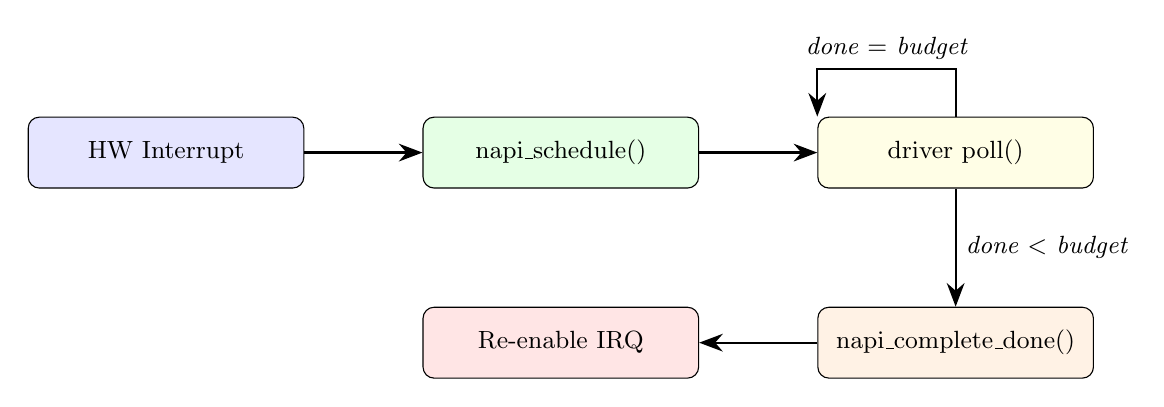
\begin{tikzpicture}[
    box/.style={draw, rounded corners, minimum width=3.5cm, minimum height=0.9cm,
                text centered, font=\small},
    arr/.style={-{Stealth[length=3mm]}, thick},
    node distance=1.5cm
]
\node[box, fill=blue!10] (irq) {HW Interrupt};
\node[box, fill=green!10, right=of irq] (sched) {napi\_schedule()};
\node[box, fill=yellow!10, right=of sched] (poll) {driver poll()};
\node[box, fill=orange!10, below=of poll] (complete) {napi\_complete\_done()};
\node[box, fill=red!10, below=of sched] (rearm) {Re-enable IRQ};

\draw[arr] (irq) -- (sched);
\draw[arr] (sched) -- (poll);
\draw[arr] (poll) -- node[right, font=\small\itshape] {done $<$ budget} (complete);
\draw[arr] (complete) -- (rearm);
\draw[arr] (poll.north) -- ++(0,0.6) -| node[above, pos=0.25, font=\small\itshape]
    {done $=$ budget} (poll.north west);
\end{tikzpicture}
\caption{NAPI poll lifecycle.  The poll function is called repeatedly
  as long as it returns \texttt{budget}; it exits the cycle by returning
  less than \texttt{budget}.}
\label{fig:napi-lifecycle}
\end{figure}

\section{The \texttt{napi\_struct}}

Each NAPI instance is represented by a \sym{napi\_struct}:

\begin{lstlisting}[caption={Simplified \texttt{napi\_struct} (include/linux/netdevice.h)}]
struct napi_struct {
    unsigned long       state;
    struct list_head    poll_list;
    int                 weight;
    int                 (*poll)(struct napi_struct *, int);
    struct net_device   *dev;
    struct hrtimer      timer;
    /* ... */
};
\end{lstlisting}

The \sym{state} field is a bitmask of flags.  The ones relevant to
this book are:

\begin{table}[H]
\centering
\begin{tabular}{lp{10cm}}
\toprule
\textbf{Flag} & \textbf{Meaning} \\
\midrule
\flag{NAPI\_STATE\_SCHED} &
    NAPI is scheduled for polling.  Set by \func{napi\_schedule\_prep},
    cleared by \func{napi\_complete\_done}.  \\
\flag{NAPI\_STATE\_MISSED} &
    New work arrived while NAPI was completing.  If
    \func{napi\_complete\_done} sees this flag, it re-schedules the
    poll instead of completing.  \\
\flag{NAPI\_STATE\_DISABLE} &
    NAPI is being disabled.  \func{napi\_schedule\_prep} will refuse
    to schedule when this is set.  \\
\bottomrule
\end{tabular}
\caption{Key NAPI state flags.}
\label{tab:napi-flags}
\end{table}

\section{The Budget Contract}
\label{sec:budget-contract}

The NAPI budget contract is the fundamental agreement between the kernel
and the driver's poll function:

\begin{itemize}
\item The kernel calls \texttt{poll(napi, budget)} with a positive
    budget (default weight is 64).
\item If the driver returns a value \textbf{equal to} \texttt{budget},
    the kernel assumes there is more work and will call \texttt{poll}
    again.
\item If the driver returns a value \textbf{less than} \texttt{budget},
    the driver must have called \func{napi\_complete\_done} to signal
    that the poll cycle is finished.
\end{itemize}

This contract is critical: if a poll function \emph{always} returns
\texttt{budget} without ever returning a smaller value, NAPI will keep
polling forever.  This is exactly what happens in the bug we are fixing.

\section{\texttt{napi\_complete\_done()}: The Completion CAS Loop}
\label{sec:napi-complete-done}

\func{napi\_complete\_done} is the function that transitions a NAPI
instance from the ``polling'' state back to the ``idle'' state.  Its
implementation contains an atomic compare-and-swap (CAS) loop that
handles the \flag{MISSED} flag:

\begin{lstlisting}[caption={\texttt{napi\_complete\_done()} core logic (net/core/dev.c)},
    label=lst:napi-complete-done]
bool napi_complete_done(struct napi_struct *n, int work_done)
{
    unsigned long flags, val, new, timeout = 0;
    bool ret = true;

    if (unlikely(n->state & (NAPIF_STATE_NPSVC |
                             NAPIF_STATE_IN_BUSY_POLL)))
        return false;

    /* ... GRO flush, poll_list removal ... */

    val = READ_ONCE(n->state);
    do {
        WARN_ON_ONCE(!(val & NAPIF_STATE_SCHED));

        new = val & ~(NAPIF_STATE_MISSED | NAPIF_STATE_SCHED |
                      NAPIF_STATE_SCHED_THREADED |
                      NAPIF_STATE_PREFER_BUSY_POLL);

        /* If MISSED was set, keep SCHED set for one more poll */
        new |= (val & NAPIF_STATE_MISSED) /
               NAPIF_STATE_MISSED * NAPIF_STATE_SCHED;
    } while (!try_cmpxchg(&n->state, &val, new));

    if (unlikely(val & NAPIF_STATE_MISSED)) {
        __napi_schedule(n);
        return false;
    }

    /* ... hrtimer for GRO ... */
    return ret;
}
\end{lstlisting}

The key insight is the \flag{MISSED} flag re-scheduling logic.  When
another CPU (or the driver itself) sets \flag{MISSED} during the CAS
window, \func{napi\_complete\_done} sees it and re-schedules NAPI
instead of completing.  This is the ``missed interrupt'' recovery
mechanism, and it is what gets exploited by the infinite loop bug.

\section{\texttt{napi\_synchronize()}: Waiting for Poll Completion}
\label{sec:napi-synchronize}

\func{napi\_synchronize} is a simple busy-wait that spins until the
\flag{NAPI\_STATE\_SCHED} bit is clear:

\begin{lstlisting}[caption={\texttt{napi\_synchronize()} (include/linux/netdevice.h)}]
static inline void napi_synchronize(const struct napi_struct *n)
{
    if (IS_ENABLED(CONFIG_SMP))
        while (test_bit(NAPI_STATE_SCHED, &n->state))
            msleep(1);
    else
        barrier();
}
\end{lstlisting}

This function does not \emph{disable} future activations---it merely
waits for the current poll cycle to end.  It is used by \func{igb\_down}
to ensure all in-flight NAPI poll callbacks have completed before
tearing down hardware resources.

\textbf{Critical property:} if the poll function never returns
\texttt{done < budget}, then \func{napi\_complete\_done} is never called,
\flag{NAPI\_STATE\_SCHED} is never cleared, and
\func{napi\_synchronize} \textbf{hangs forever}.

\section{\texttt{igb\_poll()}: The igb Driver's NAPI Callback}
\label{sec:igb-poll}

The \texttt{igb} driver registers \func{igb\_poll} as the NAPI poll
callback.  It processes TX completions first, then RX packets:

\begin{lstlisting}[caption={\texttt{igb\_poll()} (igb\_main.c:8280)},
    label=lst:igb-poll]
static int igb_poll(struct napi_struct *napi, int budget)
{
    struct igb_q_vector *q_vector = container_of(napi,
                         struct igb_q_vector, napi);
    struct xsk_buff_pool *xsk_pool;
    bool clean_complete = true;
    int work_done = 0;

    if (q_vector->tx.ring)
        clean_complete = igb_clean_tx_irq(q_vector, budget);

    if (q_vector->rx.ring) {
        int cleaned;

        xsk_pool = READ_ONCE(q_vector->rx.ring->xsk_pool);
        cleaned = xsk_pool ?
            igb_clean_rx_irq_zc(q_vector, xsk_pool, budget) :
            igb_clean_rx_irq(q_vector, budget);

        work_done += cleaned;
        if (cleaned >= budget)
            clean_complete = false;
    }

    if (!clean_complete)
        return budget;

    if (likely(napi_complete_done(napi, work_done)))
        igb_ring_irq_enable(q_vector);

    return work_done;
}
\end{lstlisting}

The decision tree is:

\begin{enumerate}
\item If \func{igb\_clean\_tx\_irq} returns \texttt{false} (more TX work),
    \texttt{clean\_complete} is set to \texttt{false}.
\item If the RX cleaner returns \texttt{budget} or more,
    \texttt{clean\_complete} is set to \texttt{false}.
\item If \texttt{clean\_complete} is \texttt{false}, return
    \texttt{budget} without calling \func{napi\_complete\_done}---NAPI
    will call us again.
\item Otherwise, call \func{napi\_complete\_done} and re-enable
    interrupts.
\end{enumerate}

\section{The \texttt{\_\_IGB\_DOWN} Early-Exit Pattern}
\label{sec:igb-down-pattern}

\func{igb\_clean\_tx\_irq} begins with an early-exit check:

\begin{lstlisting}[caption={\texttt{\_\_IGB\_DOWN} check in \texttt{igb\_clean\_tx\_irq()} (igb\_main.c:8344)},
    label=lst:tx-irq-down-check]
static bool igb_clean_tx_irq(struct igb_q_vector *q_vector,
                             int napi_budget)
{
    struct igb_adapter *adapter = q_vector->adapter;
    /* ... */

    if (test_bit(__IGB_DOWN, &adapter->state))
        return true;

    /* ... process TX completions ... */
}
\end{lstlisting}

When the adapter is going down (\flag{\_\_IGB\_DOWN} is set by
\func{igb\_down}), \func{igb\_clean\_tx\_irq} returns \texttt{true}
immediately.  In the context of \func{igb\_poll}, \texttt{true} means
``TX work is complete'' (sets \texttt{clean\_complete = true}).

This pattern is crucial: it ensures that during shutdown, the TX
cleaning path does not hold up NAPI completion.  \textbf{The bug is
that \func{igb\_clean\_rx\_irq\_zc} lacks this same check.}


% ======================================================================
\chapter{AF\_XDP Zero-Copy in igb}
\label{ch:afxdp}
% ======================================================================

AF\_XDP is a high-performance packet I/O mechanism that allows
user-space applications to send and receive network packets with minimal
kernel overhead.  When used in \emph{zero-copy mode}, the NIC's DMA
engine reads and writes directly to user-space memory, bypassing the
kernel's \texttt{sk\_buff} allocation entirely.

\section{AF\_XDP Architecture}

An AF\_XDP socket operates on a shared memory region called a UMEM
(User Memory for Efficient Mapping).  The UMEM is divided into
fixed-size frames, and four ring buffers coordinate frame ownership
between the kernel and user-space:

\begin{table}[H]
\centering
\begin{tabular}{lll}
\toprule
\textbf{Ring} & \textbf{Direction} & \textbf{Purpose} \\
\midrule
Fill Queue (FQ)      & User $\to$ Kernel & User provides empty frames for RX \\
Completion Queue (CQ)& Kernel $\to$ User & Kernel returns frames after TX \\
RX Ring              & Kernel $\to$ User & Kernel delivers received packets \\
TX Ring              & User $\to$ Kernel & User submits packets for TX \\
\bottomrule
\end{tabular}
\caption{AF\_XDP ring buffers.}
\end{table}

In zero-copy mode, the kernel maps the UMEM directly into the NIC's DMA
address space.  The driver programs the NIC's RX descriptor ring with
DMA addresses pointing into the UMEM, so received packets land directly
in user-space memory.

\section{Zero-Copy vs.\ Copy Mode}

\begin{description}
\item[Copy mode] The kernel receives packets into its own buffers via
    the normal RX path, then copies the packet data into the AF\_XDP
    socket's UMEM.  This adds a \texttt{memcpy} per packet but works
    with any driver.
\item[Zero-copy mode] The driver is aware of AF\_XDP and programs the
    NIC to DMA directly into the UMEM.  This eliminates the copy but
    requires explicit driver support.  The \texttt{igb} driver gained
    zero-copy support in commit \texttt{2c6196013f84} (``igb: Add AF\_XDP
    zero-copy Rx support'').
\end{description}

\section{The XSK Buffer Pool}

The kernel-side representation of the UMEM for a particular queue is
the \sym{xsk\_buff\_pool}.  It is created when a user-space application
binds an AF\_XDP socket to a specific queue:

\begin{lstlisting}[caption={XSK pool reference in \texttt{igb\_ring} (igb.h)}]
struct igb_ring {
    /* ... */
    struct xsk_buff_pool *xsk_pool;
    /* ... */
    union {
        struct igb_rx_buffer *rx_buffer_info;
        struct xdp_buff **rx_buffer_info_zc;
    };
    /* ... */
};
\end{lstlisting}

When the pool is present, the ring uses \sym{rx\_buffer\_info\_zc} (an
array of \sym{xdp\_buff} pointers) instead of the normal
\sym{rx\_buffer\_info}.  Buffer allocation uses \func{xsk\_buff\_alloc}
or \func{xsk\_buff\_alloc\_batch} to obtain frames from the Fill Queue.

\textbf{Key observation:} when the AF\_XDP application dies, the pool
is destroyed.  After that point, \func{xsk\_buff\_alloc} returns
\texttt{NULL}---there are no more frames to allocate.

\section{\texttt{igb\_clean\_rx\_irq\_zc()}: The Zero-Copy RX Path}
\label{sec:clean-rx-zc}

\func{igb\_clean\_rx\_irq\_zc} is the RX poll function used when a ZC
pool is active on a ring.  It is selected by \func{igb\_poll} based on
the presence of \sym{xsk\_pool}:

\begin{lstlisting}[caption={ZC RX path selection in \texttt{igb\_poll()} (igb\_main.c:8300)}]
xsk_pool = READ_ONCE(q_vector->rx.ring->xsk_pool);
cleaned = xsk_pool ?
    igb_clean_rx_irq_zc(q_vector, xsk_pool, budget) :
    igb_clean_rx_irq(q_vector, budget);
\end{lstlisting}

The function processes received packets from the descriptor ring,
runs them through the XDP program, and allocates replacement buffers
from the pool:

\begin{lstlisting}[caption={\texttt{igb\_clean\_rx\_irq\_zc()} (igb\_xsk.c:341), simplified},
    label=lst:clean-rx-zc]
int igb_clean_rx_irq_zc(struct igb_q_vector *q_vector,
                        struct xsk_buff_pool *xsk_pool,
                        const int budget)
{
    struct igb_adapter *adapter = q_vector->adapter;
    struct igb_ring *rx_ring = q_vector->rx.ring;
    unsigned int total_packets = 0;
    /* ... */

    /* NO __IGB_DOWN CHECK HERE (this is the bug) */

    xdp_prog = READ_ONCE(rx_ring->xdp_prog);

    while (likely(total_packets < budget)) {
        /* Try to read a completed RX descriptor */
        rx_desc = IGB_RX_DESC(rx_ring, ntc);
        size = le16_to_cpu(rx_desc->wb.upper.length);
        if (!size)
            break;     /* no more completed descriptors */

        /* ... process the packet via XDP ... */
        total_packets++;
    }

    /* ... update ring pointers ... */

    /* Try to refill the ring with new buffers */
    entries_to_alloc = igb_desc_unused(rx_ring);
    if (entries_to_alloc >= IGB_RX_BUFFER_WRITE)
        failure |= !igb_alloc_rx_buffers_zc(rx_ring, xsk_pool,
                                            entries_to_alloc);

    if (xsk_uses_need_wakeup(xsk_pool)) {
        /* ... wakeup handling ... */
        return (int)total_packets;
    }
    return failure ? budget : (int)total_packets;
}
\end{lstlisting}

\subsection{The Return Value Semantics}

The return value of \func{igb\_clean\_rx\_irq\_zc} determines
whether NAPI considers the poll complete:

\begin{itemize}
\item If \texttt{total\_packets < budget}, NAPI calls
    \func{napi\_complete\_done} and the poll cycle ends.
\item If \texttt{total\_packets >= budget} (or \texttt{failure}
    returns \texttt{budget}), NAPI continues polling.
\end{itemize}

The \texttt{failure} flag is set when buffer allocation fails---meaning
the Fill Queue is empty.  In that case, the function returns
\texttt{budget} to request another poll cycle, hoping that the user-space
application will refill the Fill Queue.

\subsection{What Happens When the Pool Is Destroyed}

When the AF\_XDP application dies:
\begin{enumerate}
\item The XSK buffer pool is destroyed.
\item \func{xsk\_buff\_alloc\_batch} returns 0 buffers---the Fill Queue
    is gone.
\item \func{igb\_alloc\_rx\_buffers\_zc} returns \texttt{false}
    (failure), so \texttt{failure = true}.
\item There are no completed RX descriptors (the NIC has no buffers
    to write to), so the \texttt{while} loop processes 0 packets.
\item \texttt{total\_packets = 0}, but \texttt{failure = true}, so the
    function returns \texttt{budget}.
\item Back in \func{igb\_poll}: \texttt{cleaned >= budget} $\Rightarrow$
    \texttt{clean\_complete = false} $\Rightarrow$ return \texttt{budget}
    without calling \func{napi\_complete\_done}.
\item NAPI re-schedules the poll.  Go to step 2.
\end{enumerate}

This creates an \textbf{infinite NAPI poll loop}: the function keeps
returning \texttt{budget} because it cannot allocate buffers, and NAPI
keeps calling it because it thinks there is more work to do.

\section{\texttt{igb\_xsk\_wakeup()}: The \texttt{ndo\_xsk\_wakeup} Callback}
\label{sec:xsk-wakeup}

User-space triggers NAPI polling via the \func{sendmsg} system call on
the AF\_XDP socket, which eventually calls the driver's
\sym{ndo\_xsk\_wakeup} callback.  In \texttt{igb}, this is
\func{igb\_xsk\_wakeup}:

\begin{lstlisting}[caption={\texttt{igb\_xsk\_wakeup()} (igb\_xsk.c:527)},
    label=lst:xsk-wakeup]
int igb_xsk_wakeup(struct net_device *dev, u32 qid, u32 flags)
{
    struct igb_adapter *adapter = netdev_priv(dev);
    struct e1000_hw *hw = &adapter->hw;
    struct igb_ring *ring;
    u32 eics = 0;

    if (test_bit(__IGB_DOWN, &adapter->state))
        return -ENETDOWN;

    if (!igb_xdp_is_enabled(adapter))
        return -EINVAL;

    /* ... validation ... */

    if (!napi_if_scheduled_mark_missed(
            &ring->q_vector->napi)) {
        /* Cause software interrupt */
        if (adapter->flags & IGB_FLAG_HAS_MSIX) {
            eics |= ring->q_vector->eims_value;
            wr32(E1000_EICS, eics);
        } else {
            wr32(E1000_ICS, E1000_ICS_RXDMT0);
        }
    }

    return 0;
}
\end{lstlisting}

\textbf{Important:} this function is called under \texttt{rcu\_read\_lock()}
by the AF\_XDP core.  This means that if we want to ensure no more
\func{igb\_xsk\_wakeup} calls are in flight, we need
\func{synchronize\_rcu}.  This fact becomes relevant in Patch~3
(Chapter~\ref{ch:patches}).

\section{Buffer Pool Lifecycle}

The full lifecycle of a zero-copy buffer pool:

\begin{enumerate}
\item \textbf{Creation.}  User-space creates an AF\_XDP socket and binds
    it to queue $N$.  The kernel creates an \sym{xsk\_buff\_pool} and
    stores it in \texttt{adapter->rx\_ring[N]->xsk\_pool}.
\item \textbf{Active use.}  The driver's ZC RX/TX paths use the pool to
    allocate and complete buffers.
\item \textbf{Destruction.}  The AF\_XDP socket is closed (either
    normally or because the process dies).  The pool is destroyed, and
    \texttt{xsk\_pool} is set to \texttt{NULL}---but not necessarily
    before the NAPI poll function has already read the old pointer.
\end{enumerate}

The race between pool destruction and NAPI polling is what triggers
the bug: \func{igb\_poll} reads a non-NULL \sym{xsk\_pool} pointer
and calls \func{igb\_clean\_rx\_irq\_zc}, but by the time the
function tries to allocate buffers, the pool is already gone.


% ======================================================================
\chapter{XDP Program Lifecycle and Device Reset}
\label{ch:xdp-lifecycle}
% ======================================================================

\section{\texttt{igb\_xdp\_setup()}: Installing and Removing XDP Programs}
\label{sec:xdp-setup}

The netdev core calls \func{igb\_xdp\_setup} when an XDP program is
attached to or detached from the interface.  The function handles two
cases:

\begin{description}
\item[Program replacement] (e.g., updating the XDP program without
    changing modes): the new program is atomically swapped in without
    a reset.
\item[Mode transition] (XDP $\to$ non-XDP or non-XDP $\to$ XDP): the
    device must be reset because the ring layout changes.
\end{description}

\begin{lstlisting}[caption={\texttt{igb\_xdp\_setup()} (igb\_main.c:2890)},
    label=lst:xdp-setup]
static int igb_xdp_setup(struct net_device *dev,
                         struct netdev_bpf *bpf)
{
    struct igb_adapter *adapter = netdev_priv(dev);
    struct bpf_prog *prog = bpf->prog, *old_prog;
    bool running = netif_running(dev);
    bool need_reset;

    /* ... frame size validation ... */

    old_prog = xchg(&adapter->xdp_prog, prog);
    need_reset = (!!prog != !!old_prog);

    if (need_reset && running) {
        igb_close(dev);
    } else {
        for (i = 0; i < adapter->num_rx_queues; i++)
            (void)xchg(&adapter->rx_ring[i]->xdp_prog,
                adapter->xdp_prog);
    }

    if (old_prog)
        bpf_prog_put(old_prog);

    if (!need_reset)
        return 0;

    /* ... xdp_features update ... */

    if (running)
        igb_open(dev);

    return 0;
}
\end{lstlisting}

When a mode transition occurs on a running device, the function calls
\func{igb\_close} followed by \func{igb\_open}.  This is a complete
device teardown and reinitialization---the most disruptive operation
the driver performs.

\subsection{The \texttt{xchg()} Swap}

The program pointer is swapped atomically using \func{xchg}:

\begin{lstlisting}
old_prog = xchg(&adapter->xdp_prog, prog);
\end{lstlisting}

This is an atomic read-modify-write: it stores \texttt{prog} into
\texttt{adapter->xdp\_prog} and returns the previous value.  The
\texttt{need\_reset} flag is then computed by comparing whether the
``has XDP'' state changed:

\begin{lstlisting}
need_reset = (!!prog != !!old_prog);
\end{lstlisting}

The double negation (\texttt{!!}) converts the pointer to a boolean.
If both are non-NULL (program replacement) or both are NULL (no-op),
\texttt{need\_reset} is false and no close/open is needed.

\section{\texttt{igb\_close()}: Tearing Down the Device}

\func{igb\_close} is the network device's close callback
(\texttt{ndo\_stop}).  It delegates to \func{\_\_igb\_close}:

\begin{lstlisting}[caption={\texttt{igb\_close()} and \texttt{\_\_igb\_close()} (igb\_main.c:4259)}]
static int __igb_close(struct net_device *netdev,
                       bool suspending)
{
    struct igb_adapter *adapter = netdev_priv(netdev);

    igb_down(adapter);
    igb_free_irq(adapter);
    igb_free_all_tx_resources(adapter);
    igb_free_all_rx_resources(adapter);
    /* ... */
    return 0;
}
\end{lstlisting}

The real work happens in \func{igb\_down}.

\section{\texttt{igb\_down()}: The Shutdown Sequence}
\label{sec:igb-down}

\func{igb\_down} is the core shutdown function.  Understanding its
sequence is essential for understanding the bug:

\begin{lstlisting}[caption={\texttt{igb\_down()} (igb\_main.c:2170)},
    label=lst:igb-down]
void igb_down(struct igb_adapter *adapter)
{
    struct net_device *netdev = adapter->netdev;
    struct e1000_hw *hw = &adapter->hw;

    /* (1) Signal shutdown */
    set_bit(__IGB_DOWN, &adapter->state);

    /* (2) Disable HW RX */
    rctl = rd32(E1000_RCTL);
    wr32(E1000_RCTL, rctl & ~E1000_RCTL_EN);

    /* (3) Stop TX queues, disable HW TX */
    netif_carrier_off(netdev);
    netif_tx_stop_all_queues(netdev);
    tctl = rd32(E1000_TCTL);
    tctl &= ~E1000_TCTL_EN;
    wr32(E1000_TCTL, tctl);
    wrfl();
    usleep_range(10000, 11000);

    /* (4) Disable interrupts */
    igb_irq_disable(adapter);

    /* (5) Wait for NAPI, then disable it */
    for (i = 0; i < adapter->num_q_vectors; i++) {
        if (adapter->q_vector[i]) {
            napi_synchronize(
                &adapter->q_vector[i]->napi);
            napi_disable(
                &adapter->q_vector[i]->napi);
        }
    }

    /* (6) Cancel timers, update stats, reset HW */
    timer_delete_sync(&adapter->watchdog_timer);
    /* ... */
    igb_reset(adapter);

    /* (7) Clean all rings */
    igb_clean_all_tx_rings(adapter);
    igb_clean_all_rx_rings(adapter);
}
\end{lstlisting}

The sequence has a clear dependency chain:

\begin{enumerate}
\item \textbf{Set \flag{\_\_IGB\_DOWN}} (step 1) to signal all paths that
    the adapter is going down.
\item \textbf{Disable hardware} (steps 2--4) to stop new packets and
    interrupts.
\item \textbf{Wait for NAPI} (step 5): \func{napi\_synchronize} blocks
    until the current poll cycle completes, then \func{napi\_disable}
    prevents future scheduling.
\item \textbf{Clean up} (steps 6--7) now that no concurrent access is
    possible.
\end{enumerate}

\textbf{The critical point:} step 5 can \emph{only} proceed if the poll
function eventually returns \texttt{done < budget}.  If the poll
function is stuck in an infinite loop (as with the ZC bug), step 5
hangs forever, and steps 6--7 never execute.

\section{\texttt{igb\_up()} and \texttt{\_\_igb\_open()}: Bringing the Device Up}
\label{sec:igb-up}

\func{igb\_up} (and its more complete sibling \func{\_\_igb\_open}) reverses
the shutdown:

\begin{lstlisting}[caption={\texttt{igb\_up()} key steps (igb\_main.c:2122)}]
int igb_up(struct igb_adapter *adapter)
{
    /* (1) Configure hardware */
    igb_configure(adapter);

    /* (2) Clear shutdown flag */
    clear_bit(__IGB_DOWN, &adapter->state);

    /* (3) Enable NAPI */
    for (i = 0; i < adapter->num_q_vectors; i++) {
        napi = &adapter->q_vector[i]->napi;
        napi_enable(napi);
    }

    /* (4) Enable interrupts and start TX queues */
    igb_irq_enable(adapter);
    netif_tx_start_all_queues(adapter->netdev);

    /* (5) Start watchdog */
    schedule_work(&adapter->watchdog_task);

    return 0;
}
\end{lstlisting}

The \flag{\_\_IGB\_DOWN} bit is cleared \emph{after} configuration but
\emph{before} enabling NAPI and starting TX queues.

\section{\texttt{igb\_reinit\_locked()}: The Reset Helper}

\func{igb\_reinit\_locked} is a convenience wrapper that performs
\func{igb\_down} + \func{igb\_up} while holding the \flag{\_\_IGB\_RESETTING}
flag:

\begin{lstlisting}[caption={\texttt{igb\_reinit\_locked()} (igb\_main.c:2238)}]
void igb_reinit_locked(struct igb_adapter *adapter)
{
    while (test_and_set_bit(__IGB_RESETTING,
                            &adapter->state))
        usleep_range(1000, 2000);
    igb_down(adapter);
    igb_up(adapter);
    clear_bit(__IGB_RESETTING, &adapter->state);
}
\end{lstlisting}

This is called by \func{igb\_reset\_task} (the workqueue handler
for TX timeouts) and various reconfiguration paths.

\section{The Close/Open Window}
\label{sec:close-open-window}

When \func{igb\_xdp\_setup} calls \func{igb\_close} followed by
\func{igb\_open}, there is a window during which:

\begin{enumerate}
\item The adapter is down (\flag{\_\_IGB\_DOWN} is set).
\item All TX queues are stopped (\func{netif\_tx\_stop\_all\_queues}).
\item The TX watchdog timer may still be armed from before the close.
\item The \texttt{trans\_start} timestamps on the TX queues are stale
    (they reflect the last transmission \emph{before} the close).
\end{enumerate}

This window is where the TX watchdog can fire a spurious timeout,
because it sees stopped queues with stale timestamps.


% ======================================================================
\chapter{TX Watchdog and Timeout Handling}
\label{ch:watchdog}
% ======================================================================

\section{\texttt{dev\_watchdog()}: The Network TX Watchdog Timer}

The Linux kernel maintains a per-device watchdog timer that monitors TX
queue health.  The timer callback, \func{dev\_watchdog}, fires
periodically and checks whether any \emph{stopped} TX queue has exceeded
its timeout:

\begin{lstlisting}[caption={\texttt{dev\_watchdog()} (net/sched/sch\_generic.c:500), simplified}]
static void dev_watchdog(struct timer_list *t)
{
    struct net_device *dev = /* ... */;

    if (netif_device_present(dev) &&
        netif_running(dev) &&
        netif_carrier_ok(dev)) {

        for (i = 0; i < dev->num_tx_queues; i++) {
            txq = netdev_get_tx_queue(dev, i);
            if (!netif_xmit_stopped(txq))
                continue;

            trans_start = READ_ONCE(txq->trans_start);

            if (time_after(jiffies,
                    trans_start + dev->watchdog_timeo)) {
                /* TIMEOUT! */
                netdev_crit(dev,
                    "NETDEV WATCHDOG: CPU: %d: "
                    "transmit queue %u timed out "
                    "%u ms\n", ...);
                dev->netdev_ops->ndo_tx_timeout(dev, i);
            }
        }
    }
}
\end{lstlisting}

The default \texttt{watchdog\_timeo} is 5 seconds (\texttt{5*HZ}).
The watchdog only checks queues that are \emph{stopped}---if a queue
is actively transmitting, its \texttt{trans\_start} is continuously
updated and the watchdog never fires.

\subsection{The Conditions for a TX Timeout}

All of the following must be true for the watchdog to fire:

\begin{enumerate}
\item The device is present, running, and has carrier.
\item A TX queue is stopped (via \func{netif\_stop\_subqueue} or
    \func{netif\_tx\_stop\_all\_queues}).
\item The queue's \texttt{trans\_start} timestamp is more than
    \texttt{watchdog\_timeo} jiffies in the past.
\end{enumerate}

\section{\texttt{igb\_tx\_timeout()}: The Driver's Timeout Handler}

When the watchdog detects a timeout, it calls the driver's
\sym{ndo\_tx\_timeout} callback.  In \texttt{igb}, this is
\func{igb\_tx\_timeout}:

\begin{lstlisting}[caption={\texttt{igb\_tx\_timeout()} before patches (igb\_main.c:6649)}]
static void igb_tx_timeout(struct net_device *netdev,
              unsigned int __always_unused txqueue)
{
    struct igb_adapter *adapter = netdev_priv(netdev);
    struct e1000_hw *hw = &adapter->hw;

    /* Do the reset outside of interrupt context */
    adapter->tx_timeout_count++;

    if (hw->mac.type >= e1000_82580)
        hw->dev_spec._82575.global_device_reset = true;

    schedule_work(&adapter->reset_task);
    wr32(E1000_EICS,
         (adapter->eims_enable_mask & ~adapter->eims_other));
}
\end{lstlisting}

The handler does two things:
\begin{enumerate}
\item Schedules \func{igb\_reset\_task} on a workqueue, which will call
    \func{igb\_reinit\_locked} (= \func{igb\_down} + \func{igb\_up}).
\item Triggers a software interrupt to attempt to flush any stuck
    descriptors.
\end{enumerate}

\section{\texttt{igb\_reset\_task()}: The Reset Workqueue Handler}

\begin{lstlisting}[caption={\texttt{igb\_reset\_task()} (igb\_main.c:6665)}]
static void igb_reset_task(struct work_struct *work)
{
    struct igb_adapter *adapter;
    adapter = container_of(work, struct igb_adapter,
                           reset_task);

    rtnl_lock();
    /* If we're already down or resetting, just bail */
    if (test_bit(__IGB_DOWN, &adapter->state) ||
        test_bit(__IGB_RESETTING, &adapter->state)) {
        rtnl_unlock();
        return;
    }

    igb_dump(adapter);
    netdev_err(adapter->netdev, "Reset adapter\n");
    igb_reinit_locked(adapter);
    rtnl_unlock();
}
\end{lstlisting}

Note that \func{igb\_reset\_task} \emph{does} check \flag{\_\_IGB\_DOWN}
before proceeding.  However, this check races with the timeout
detection: the watchdog fires, \func{igb\_tx\_timeout} calls
\func{schedule\_work}, and by the time the work item runs, the
adapter state may have changed.  The work item may already be
queued and waiting to run---and it will run \emph{after}
\func{igb\_open} completes in the XDP transition path.

\section{\texttt{trans\_start} and \texttt{txq\_trans\_cond\_update()}}

The per-queue timestamp \texttt{trans\_start} is updated by the
transmit path each time a packet is queued:

\begin{lstlisting}[caption={\texttt{txq\_trans\_cond\_update()} (include/linux/netdevice.h)}]
static inline void txq_trans_cond_update(
    struct netdev_queue *txq)
{
    unsigned long now = jiffies;
    if (READ_ONCE(txq->trans_start) != now)
        WRITE_ONCE(txq->trans_start, now);
}
\end{lstlisting}

The legacy single-queue helper \func{netif\_trans\_update} updates
queue 0's \texttt{trans\_start}:

\begin{lstlisting}[caption={\texttt{netif\_trans\_update()} (include/linux/netdevice.h)}]
static inline void netif_trans_update(struct net_device *dev)
{
    struct netdev_queue *txq = netdev_get_tx_queue(dev, 0);
    txq_trans_cond_update(txq);
}
\end{lstlisting}

\section{The Stale Timestamp Problem}
\label{sec:stale-timestamp}

During the close/open transition in \func{igb\_xdp\_setup}:

\begin{enumerate}
\item \func{igb\_close} calls \func{igb\_down}, which calls
    \func{netif\_tx\_stop\_all\_queues}.  The TX queues are now stopped.
\item The \texttt{trans\_start} values still reflect the last
    transmission \emph{before} the close.  No code updates them.
\item The TX watchdog timer may have been armed before the close and
    fires during the close/open window.
\item The watchdog sees: stopped queues + stale \texttt{trans\_start}
    that is more than 5 seconds old = \textbf{timeout}.
\item \func{igb\_tx\_timeout} schedules \func{igb\_reset\_task}.
\end{enumerate}

This is a false positive: the queues are stopped because the device is
being reconfigured, not because of a hardware hang.  But the timeout
handler does not distinguish between the two cases.

\begin{figure}[H]
\centering
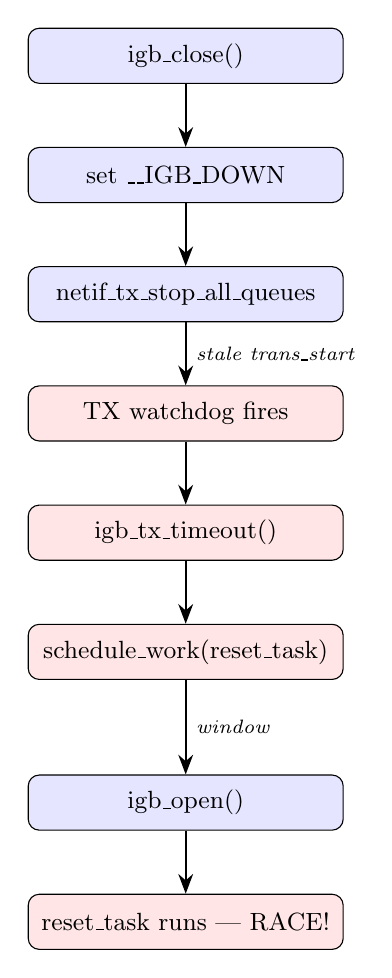
\begin{tikzpicture}[
    event/.style={draw, fill=blue!10, rounded corners, minimum width=4cm,
                  minimum height=0.7cm, font=\small, text centered},
    problem/.style={draw, fill=red!10, rounded corners, minimum width=4cm,
                    minimum height=0.7cm, font=\small, text centered},
    arr/.style={-{Stealth[length=2.5mm]}, thick},
    node distance=0.8cm
]
\node[event] (close) {igb\_close()};
\node[event, below=of close] (down) {set \_\_IGB\_DOWN};
\node[event, below=of down] (stop) {netif\_tx\_stop\_all\_queues};
\node[problem, below=of stop] (wd) {TX watchdog fires};
\node[problem, below=of wd] (timeout) {igb\_tx\_timeout()};
\node[problem, below=of timeout] (sched) {schedule\_work(reset\_task)};
\node[event, below=1.2cm of sched] (open) {igb\_open()};
\node[problem, below=of open] (reset) {reset\_task runs --- RACE!};

\draw[arr] (close) -- (down);
\draw[arr] (down) -- (stop);
\draw[arr] (stop) -- node[right, font=\scriptsize\itshape] {stale trans\_start} (wd);
\draw[arr] (wd) -- (timeout);
\draw[arr] (timeout) -- (sched);
\draw[arr] (sched) -- node[right, font=\scriptsize\itshape] {window} (open);
\draw[arr] (open) -- (reset);
\end{tikzpicture}
\caption{The stale timestamp race during XDP close/open transition.}
\label{fig:stale-timestamp}
\end{figure}


% ======================================================================
\chapter{The Patch Series---Analysis and Correctness}
\label{ch:patches}
% ======================================================================

This chapter analyzes each of the three patches in the fix series.
For each patch, we describe the root cause, the fix, and why it is
correct and sufficient.

\section{Patch 1: \texttt{\_\_IGB\_DOWN} Check in \texttt{igb\_clean\_rx\_irq\_zc()}}
\label{sec:patch1}

\subsection{Commit Message}

\begin{Verbatim}[fontsize=\small]
igb: check __IGB_DOWN in igb_clean_rx_irq_zc()

When an AF_XDP zero-copy application terminates abruptly (e.g.,
kill -9), the XSK buffer pool is destroyed but NAPI polling
continues. igb_clean_rx_irq_zc() keeps returning budget (no
descriptors, no buffers to allocate, xsk_buff_alloc() returns
NULL) which makes napi_complete_done() re-arm the poll
indefinitely.

Meanwhile, igb_down() -> napi_synchronize() waits for a NAPI
poll cycle that signals completion with done < budget -- which
never happens. This blocks igb_down() forever, and the 5-second
TX watchdog fires because no TX completions are processed while
NAPI is stuck.

Fix this by adding an __IGB_DOWN check at the top of
igb_clean_rx_irq_zc(), returning 0 immediately when the adapter
is going down.

Fixes: 2c6196013f84 ("igb: Add AF_XDP zero-copy Rx support")
\end{Verbatim}

\subsection{Root Cause Analysis}

The root cause is a missing early-exit check in
\func{igb\_clean\_rx\_irq\_zc}.  Let's trace the exact sequence of
events:

\begin{enumerate}
\item An AF\_XDP zero-copy application is running on queue 0 with an
    XDP program attached.
\item The application is killed (\texttt{kill -9}).
\item The AF\_XDP socket closes, destroying the XSK buffer pool.
\item The XDP program is detached (either by the dying process or by
    the administrator).
\item \func{igb\_xdp\_setup} is called with \texttt{prog = NULL} and
    \texttt{need\_reset = true}.
\item \func{igb\_close} is called, which calls \func{igb\_down}.
\item \func{igb\_down} sets \flag{\_\_IGB\_DOWN} and eventually calls
    \func{napi\_synchronize} (step 5 in Section~\ref{sec:igb-down}).
\item But NAPI is stuck: \func{igb\_clean\_rx\_irq\_zc} keeps returning
    \texttt{budget} because:
    \begin{itemize}
    \item No RX descriptors are completed (NIC has no buffers).
    \item Buffer refill fails (\texttt{failure = true}).
    \item The function returns \texttt{budget} on failure.
    \end{itemize}
\item \func{napi\_synchronize} waits for \flag{NAPI\_STATE\_SCHED} to
    clear, but it never does because the poll function never returns
    \texttt{done < budget}.
\item \func{igb\_down} hangs at step 5.
\item Meanwhile, \func{igb\_clean\_tx\_irq} is also not processing TX
    completions (it returns \texttt{true} immediately due to its own
    \flag{\_\_IGB\_DOWN} check, but the NAPI poll loop is dominated by
    the RX side returning \texttt{budget}).
\item After 5 seconds, the TX watchdog fires because no TX completions
    have been processed and \texttt{trans\_start} is stale.
\item \func{igb\_tx\_timeout} schedules a reset, but the reset cannot
    proceed because \func{igb\_down} is already hung.
\item The TX queue is permanently stalled.
\end{enumerate}

\subsection{The Fix}

\begin{lstlisting}[caption={Patch 1 diff (igb\_xsk.c)}, style=diffstyle]
 int igb_clean_rx_irq_zc(struct igb_q_vector *q_vector,
                         struct xsk_buff_pool *xsk_pool,
                         const int budget)
 {
     struct igb_adapter *adapter = q_vector->adapter;
     /* ... */

@@+    if (test_bit(__IGB_DOWN, &adapter->state))+@@
@@+        return 0;+@@

     /* xdp_prog cannot be NULL in the ZC path */
     xdp_prog = READ_ONCE(rx_ring->xdp_prog);
\end{lstlisting}

The fix adds a single check: if \flag{\_\_IGB\_DOWN} is set, return 0
immediately.

\subsection{Why It Is Correct}

\begin{enumerate}
\item \textbf{Returns 0, not \texttt{budget}.}  Returning 0 means
    ``no work done, poll is complete.''  In \func{igb\_poll}, this
    results in \texttt{cleaned = 0 < budget}, so
    \texttt{clean\_complete} remains \texttt{true}, and
    \func{napi\_complete\_done} is called.

\item \textbf{Matches the existing pattern.}  \func{igb\_clean\_tx\_irq}
    already has the same check at line 8344, returning \texttt{true}
    (``TX complete'') when \flag{\_\_IGB\_DOWN} is set.  This patch
    extends the pattern to the ZC RX path.

\item \textbf{Breaks the infinite loop.}  With this check, once
    \func{igb\_down} sets \flag{\_\_IGB\_DOWN}, the very next poll
    cycle will have both TX and RX returning ``done,'' so
    \func{napi\_complete\_done} is called, \flag{NAPI\_STATE\_SCHED}
    is cleared, and \func{napi\_synchronize} returns.

\item \textbf{No spurious packet loss.}  When \flag{\_\_IGB\_DOWN} is set,
    the hardware RX and TX are already disabled.  No new packets will
    arrive, and any remaining descriptors will be cleaned by
    \func{igb\_clean\_all\_rx\_rings} in step 7 of \func{igb\_down}.
    Returning 0 does not lose any packets.

\item \textbf{Safe to call at any point.}  The \texttt{test\_bit} is a
    plain atomic read with no side effects.  It does not take any locks
    or modify any state.
\end{enumerate}

\subsection{What About the Normal (Non-ZC) RX Path?}

The normal RX path (\func{igb\_clean\_rx\_irq}) does \emph{not} have
this bug because it does not depend on a buffer pool.  When there are
no packets to process, it returns 0 (no packets cleaned), which is less
than the budget.  The ZC path is different because it returns
\texttt{budget} on allocation failure, creating the infinite loop.


\section{Patch 2: \texttt{\_\_IGB\_DOWN} Check in \texttt{igb\_tx\_timeout()}}
\label{sec:patch2}

\subsection{Commit Message}

\begin{Verbatim}[fontsize=\small]
igb: skip reset in igb_tx_timeout() during XDP transition

When igb_xdp_setup() transitions between XDP and non-XDP mode on
a running device, it calls igb_close() followed by igb_open().
During this window the adapter is down and trans_start is stale,
so the TX watchdog can fire a spurious timeout.

The resulting schedule_work(&adapter->reset_task) races with the
igb_open() path: the reset task may run while the device is
being brought back up, or immediately after, causing unexpected
ring reinitialisation and register writes.

Fix this by checking __IGB_DOWN at the top of igb_tx_timeout().
\end{Verbatim}

\subsection{Root Cause Analysis}

During the \func{igb\_xdp\_setup} close/open transition:

\begin{enumerate}
\item \func{igb\_close} calls \func{igb\_down}, which sets
    \flag{\_\_IGB\_DOWN} and stops all TX queues.
\item The TX watchdog timer was armed before the close and fires during
    the transition window (or shortly after).
\item \func{dev\_watchdog} sees stopped queues with stale
    \texttt{trans\_start} $\Rightarrow$ calls \func{igb\_tx\_timeout}.
\item \func{igb\_tx\_timeout} unconditionally schedules
    \func{igb\_reset\_task} via \func{schedule\_work}.
\item The reset work item may execute:
    \begin{itemize}
    \item While \func{igb\_open} is still in progress (racing with
        ring setup).
    \item After \func{igb\_open} completes (causing an unnecessary
        second reset).
    \end{itemize}
\end{enumerate}

Although \func{igb\_reset\_task} does check \flag{\_\_IGB\_DOWN} before
calling \func{igb\_reinit\_locked}, this check is not sufficient because
\texttt{reset\_task} is a work item that may not execute until after
the XDP transition completes (by which time \flag{\_\_IGB\_DOWN} has been
cleared by \func{igb\_open}).

\subsection{The Fix}

\begin{lstlisting}[caption={Patch 2 diff (igb\_main.c)}, style=diffstyle]
 static void igb_tx_timeout(struct net_device *netdev,
               unsigned int __always_unused txqueue)
 {
     struct igb_adapter *adapter = netdev_priv(netdev);
     struct e1000_hw *hw = &adapter->hw;

@@+    /* Do not schedule a reset if the adapter is+@@
@@+     * already going down or being reconfigured.+@@
@@+     */+@@
@@+    if (test_bit(__IGB_DOWN, &adapter->state))+@@
@@+        return;+@@

     /* Do the reset outside of interrupt context */
     adapter->tx_timeout_count++;
     /* ... */
     schedule_work(&adapter->reset_task);
\end{lstlisting}

\subsection{Why It Is Correct}

\begin{enumerate}
\item \textbf{Prevents spurious reset scheduling.}  When the adapter is
    down (either shutting down or in the XDP transition window), a TX
    timeout is expected and not indicative of a hardware problem.
    Scheduling a reset is pointless: the subsequent \func{igb\_open}
    will reinitialize everything.

\item \textbf{Does not mask real timeouts.}  Real TX hangs occur when
    the adapter is \emph{up} and running.  The \flag{\_\_IGB\_DOWN}
    check only suppresses timeouts during shutdown and reconfiguration,
    when timeouts are known to be false positives.

\item \textbf{Eliminates the race with \func{igb\_open}.}  By not
    scheduling the reset work item, we avoid the race where
    \func{igb\_reset\_task} runs concurrently with or after
    \func{igb\_open}.

\item \textbf{Consistent with \func{igb\_reset\_task}.}
    \func{igb\_reset\_task} already checks \flag{\_\_IGB\_DOWN} and bails
    out.  This patch moves the guard one step earlier---to the point
    where the work is scheduled---to prevent the work item from being
    queued at all.

\item \textbf{No counter increment on spurious timeout.}  By returning
    before \texttt{adapter->tx\_timeout\_count++}, we avoid inflating
    the timeout counter with false positives, which could confuse
    monitoring tools.
\end{enumerate}

\subsection{Why Not Just Rely on \texttt{igb\_reset\_task}'s Check?}

One might ask: \func{igb\_reset\_task} already checks \flag{\_\_IGB\_DOWN}
and returns early.  Why add another check in \func{igb\_tx\_timeout}?

The answer is \textbf{timing}.  \func{igb\_reset\_task} is a work item
that runs asynchronously.  Between the time it is scheduled and the
time it runs, the XDP transition may complete:

\begin{enumerate}
\item \func{igb\_tx\_timeout} schedules \func{reset\_task} (adapter is
    down, \flag{\_\_IGB\_DOWN} is set).
\item \func{igb\_xdp\_setup} completes: \func{igb\_open} clears
    \flag{\_\_IGB\_DOWN}.
\item \func{reset\_task} runs: \flag{\_\_IGB\_DOWN} is now clear, so it
    proceeds with \func{igb\_reinit\_locked}, performing an unnecessary
    and potentially disruptive reset.
\end{enumerate}

By checking \flag{\_\_IGB\_DOWN} in \func{igb\_tx\_timeout} itself, we
prevent the work item from ever being queued during the transition window.


\section{Patch 3: XDP Transition Guards in \texttt{igb\_xdp\_setup()}}
\label{sec:patch3}

\subsection{Commit Message}

\begin{Verbatim}[fontsize=\small]
igb: add XDP transition guards in igb_xdp_setup()

igb_xdp_setup() calls igb_close() + igb_open() when
transitioning between XDP and non-XDP mode on a running device.
This has two issues:

1. When removing an XDP program that has AF_XDP zero-copy
   sockets, ndo_xsk_wakeup() may be executing concurrently under
   rcu_read_lock(). If igb_close() tears down the rings while
   ndo_xsk_wakeup() is still accessing them, it races with the
   teardown. Add synchronize_rcu() before igb_close() when
   removing an XDP program.

2. The igb_close()/igb_open() window leaves trans_start stale.
   Add netif_trans_update() after igb_open() to refresh the
   timestamp, and cancel_work() to drain any reset_task queued
   during the window.
\end{Verbatim}

\subsection{The Three Sub-fixes}

Patch 3 contains three logically distinct fixes, all applied to
\func{igb\_xdp\_setup}:

\subsubsection{Fix 3a: \texttt{synchronize\_rcu()} Before Close}

\begin{lstlisting}[caption={Fix 3a: RCU synchronization (igb\_main.c)}, style=diffstyle]
     if (need_reset && running) {
@@+        if (!prog)+@@
@@+            /* Wait until ndo_xsk_wakeup completes. */+@@
@@+            synchronize_rcu();+@@
         igb_close(dev);
\end{lstlisting}

\textbf{Root cause:} \func{igb\_xsk\_wakeup} is called under
\texttt{rcu\_read\_lock()} by the AF\_XDP core.  When removing an XDP
program (\texttt{prog = NULL}), any in-flight \func{igb\_xsk\_wakeup}
calls may still be accessing the adapter's rings, interrupt registers,
and NAPI state.  If \func{igb\_close} tears down these resources while
\func{igb\_xsk\_wakeup} is running, we get a use-after-free or register
access on disabled hardware.

\textbf{Why the fix is correct:}

\begin{itemize}
\item \func{synchronize\_rcu} waits for all existing RCU read-side
    critical sections to complete.  Since \func{igb\_xsk\_wakeup} runs
    under \texttt{rcu\_read\_lock()}, this ensures all in-flight wakeup
    calls have returned before we proceed to \func{igb\_close}.
\item The condition \texttt{!prog} ensures we only synchronize when
    \emph{removing} an XDP program.  When \emph{adding} a program, there
    are no AF\_XDP sockets yet (you cannot bind a ZC socket without an
    XDP program), so the race does not exist.
\item \func{synchronize\_rcu} may sleep, but \func{igb\_xdp\_setup} is
    called from process context (under RTNL lock), so sleeping is safe.
\end{itemize}

\subsubsection{Fix 3b: \texttt{netif\_trans\_update()} After Open}

\begin{lstlisting}[caption={Fix 3b: Timestamp refresh (igb\_main.c)}, style=diffstyle]
     if (running)
         igb_open(dev);

@@+    if (need_reset && running) {+@@
@@+        netif_trans_update(dev);+@@
\end{lstlisting}

\textbf{Root cause:} After \func{igb\_open} completes, the TX queues
are started but \texttt{trans\_start} still has the stale value from
before \func{igb\_close}.  If the watchdog timer fires before the next
actual transmission, it sees the stale timestamp and triggers a false
timeout.

\textbf{Why the fix is correct:}

\begin{itemize}
\item \func{netif\_trans\_update} sets \texttt{trans\_start} on TX
    queue 0 to the current \texttt{jiffies}.  This prevents the watchdog
    from seeing a stale timestamp.
\item For the I210/I211 (which typically has a single TX queue), updating
    queue 0 is sufficient.
\item The update happens after \func{igb\_open}, so the TX queue is
    already started and the timestamp is meaningful.
\end{itemize}

\subsubsection{Fix 3c: \texttt{cancel\_work(\&adapter->reset\_task)}}

\begin{lstlisting}[caption={Fix 3c: Cancel stale reset work (igb\_main.c)}, style=diffstyle]
@@+        cancel_work(&adapter->reset_task);+@@
@@+    }+@@

     return 0;
 }
\end{lstlisting}

\textbf{Root cause:} Even with Patch~2's guard in \func{igb\_tx\_timeout},
there is a small window where a timeout could fire and schedule a
\func{reset\_task} before the \flag{\_\_IGB\_DOWN} bit is checked.  Or a
timeout could have been scheduled from a previous event.  This stale
work item would run after \func{igb\_open} and cause an unnecessary
reset.

\textbf{Why the fix is correct:}

\begin{itemize}
\item \func{cancel\_work} (a variant of \func{cancel\_work\_sync})
    ensures that any queued \func{reset\_task} is cancelled and, if it
    is currently executing, waits for it to complete.
\item This is a belt-and-suspenders approach: Patch~2 prevents most
    spurious scheduling, and this \func{cancel\_work} catches anything
    that slipped through the cracks.
\item Placing it after \func{igb\_open} ensures the device is fully up
    before we drain the work queue, so we don't accidentally cancel a
    legitimate reset.
\end{itemize}

\section{How the Three Patches Work Together}

The three patches form a defense-in-depth strategy against the
close/open transition bugs:

\begin{figure}[H]
\centering
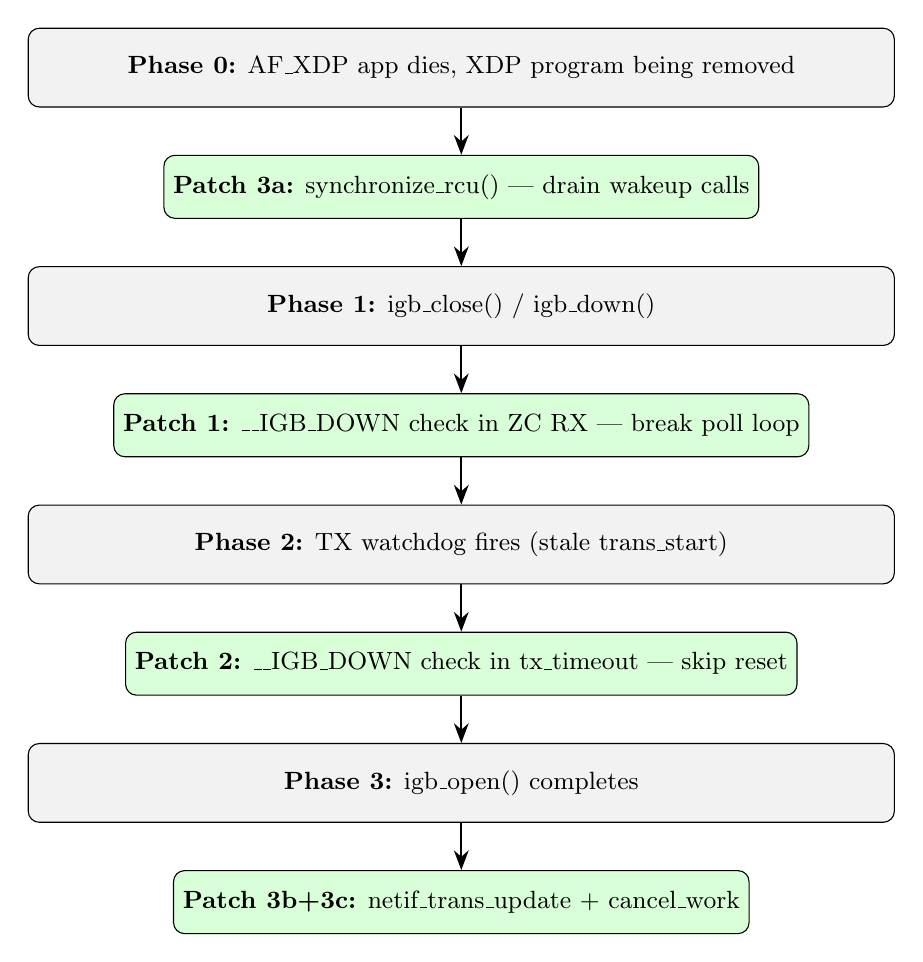
\begin{tikzpicture}[
    phase/.style={draw, fill=gray!10, rounded corners, minimum width=11cm,
                  minimum height=1cm, font=\small},
    fix/.style={draw, fill=green!15, rounded corners, minimum width=5cm,
                minimum height=0.8cm, font=\small},
    arr/.style={-{Stealth[length=2.5mm]}, thick},
    node distance=0.6cm
]
\node[phase] (p0) {\textbf{Phase 0:} AF\_XDP app dies, XDP program being removed};
\node[fix, below=of p0] (f3a)
    {\textbf{Patch 3a:} synchronize\_rcu() --- drain wakeup calls};
\node[phase, below=of f3a] (p1) {\textbf{Phase 1:} igb\_close() / igb\_down()};
\node[fix, below=of p1] (f1)
    {\textbf{Patch 1:} \_\_IGB\_DOWN check in ZC RX --- break poll loop};
\node[phase, below=of f1] (p2) {\textbf{Phase 2:} TX watchdog fires (stale trans\_start)};
\node[fix, below=of p2] (f2)
    {\textbf{Patch 2:} \_\_IGB\_DOWN check in tx\_timeout --- skip reset};
\node[phase, below=of f2] (p3) {\textbf{Phase 3:} igb\_open() completes};
\node[fix, below=of p3] (f3bc)
    {\textbf{Patch 3b+3c:} netif\_trans\_update + cancel\_work};

\draw[arr] (p0) -- (f3a);
\draw[arr] (f3a) -- (p1);
\draw[arr] (p1) -- (f1);
\draw[arr] (f1) -- (p2);
\draw[arr] (p2) -- (f2);
\draw[arr] (f2) -- (p3);
\draw[arr] (p3) -- (f3bc);
\end{tikzpicture}
\caption{The three patches address different phases of the XDP transition.}
\label{fig:patch-phases}
\end{figure}

\begin{description}[style=nextline]
\item[Patch 1 (the critical fix)]
    Breaks the infinite NAPI poll loop that causes \func{igb\_down} to
    hang.  Without this patch, nothing else matters because the driver
    is stuck forever.

\item[Patch 2 (secondary defense)]
    Prevents the TX watchdog from scheduling a spurious reset during
    the transition.  This is important even with Patch~1 because the
    watchdog can still fire due to the stale \texttt{trans\_start} during
    the close/open window.

\item[Patch 3 (transition hardening)]
    Addresses three remaining race conditions:
    \begin{itemize}
    \item RCU synchronization prevents use-after-free in
        \func{igb\_xsk\_wakeup}.
    \item Timestamp refresh prevents false timeouts after the transition.
    \item Work cancellation catches any stale reset work items.
    \end{itemize}
\end{description}

\section{Testing}

The patch series was tested on an Intel I210 controller with the
following scenarios:

\begin{enumerate}
\item \textbf{Attach XDP program, run AF\_XDP app, kill -9.}
    Before patches: permanent TX stall, requires reboot.
    After patches: clean recovery, interface returns to normal operation.

\item \textbf{Detach XDP program while AF\_XDP is running.}
    Before patches: TX stall and/or kernel oops.
    After patches: clean recovery.

\item \textbf{Repeated attach/detach cycles.}
    Before patches: intermittent stalls and timeouts.
    After patches: stable operation across hundreds of cycles.
\end{enumerate}


% ══════════════════════════════════════════════════════════════════════
%  APPENDICES
% ══════════════════════════════════════════════════════════════════════
\appendix

% ======================================================================
\chapter{Full Patch Listing}
\label{app:patches}
% ======================================================================

This appendix contains the verbatim patch files as they would be
submitted to the Linux kernel mailing list.

\section{Patch 0/3: Cover Letter}

\begin{Verbatim}[fontsize=\scriptsize, frame=single]
From: Alex Dvoretsky <advoretsky@gmail.com>
Date: Sat, 14 Feb 2026 23:11:59 +0100
Subject: [PATCH net 0/3] igb: fix TX queue stall on XDP program
 removal with AF_XDP zero-copy

Killing an AF_XDP zero-copy application while the XDP program is still
attached causes a permanent TX queue 0 stall on igb. The interface
becomes unresponsive (no ping, no SSH) and requires a reboot or
module reload to recover.

Root cause: igb_clean_rx_irq_zc() has no __IGB_DOWN check, so when the
XSK buffer pool is destroyed (process dies) but NAPI keeps polling, the
function returns budget every time. This prevents napi_complete_done()
from signaling completion, which blocks napi_synchronize() in igb_down()
indefinitely. The 5-second TX watchdog then fires because TX completions
are not processed while NAPI is stuck.

The series has three patches:

1. Add __IGB_DOWN check in igb_clean_rx_irq_zc() -- breaks the infinite
   NAPI poll loop, matching the pattern in igb_clean_tx_irq().

2. Add __IGB_DOWN check in igb_tx_timeout() -- prevents spurious
   reset_task scheduling during the igb_close()/igb_open() window in
   XDP transitions.

3. Add RCU synchronization and TX watchdog guards in igb_xdp_setup() --
   ensures ndo_xsk_wakeup() completes before teardown and prevents
   false TX timeouts from stale trans_start.

Tested on Intel I210 (igb) with AF_XDP zero-copy sockets:
- Attach XDP program, run AF_XDP app, kill -9 -> no TX stall
- Detach XDP program while AF_XDP is running -> clean recovery
- Repeated attach/detach cycles -> stable

Alex Dvoretsky (3):
  igb: check __IGB_DOWN in igb_clean_rx_irq_zc()
  igb: skip reset in igb_tx_timeout() during XDP transition
  igb: add XDP transition guards in igb_xdp_setup()

 drivers/net/ethernet/intel/igb/igb_main.c | 22 ++++++++++++++++++++++
 drivers/net/ethernet/intel/igb/igb_xsk.c  |  3 +++
 2 files changed, 25 insertions(+)
\end{Verbatim}

\section{Patch 1/3: \texttt{igb\_clean\_rx\_irq\_zc} \texttt{\_\_IGB\_DOWN} Check}

\begin{Verbatim}[fontsize=\scriptsize, frame=single]
From: Alex Dvoretsky <advoretsky@gmail.com>
Date: Sat, 14 Feb 2026 23:09:31 +0100
Subject: [PATCH net 1/3] igb: check __IGB_DOWN in igb_clean_rx_irq_zc()

When an AF_XDP zero-copy application terminates abruptly (e.g.,
kill -9), the XSK buffer pool is destroyed but NAPI polling continues.
igb_clean_rx_irq_zc() keeps returning budget (no descriptors, no
buffers to allocate, xsk_buff_alloc() returns NULL) which makes
napi_complete_done() re-arm the poll indefinitely.

Meanwhile, igb_down() -> napi_synchronize() waits for a NAPI poll cycle
that signals completion with done < budget -- which never happens. This
blocks igb_down() forever, and the 5-second TX watchdog fires because
no TX completions are processed while NAPI is stuck. Since igb_down()
never finishes, igb_up() is never called, and the TX queue remains
permanently stalled.

Fix this by adding an __IGB_DOWN check at the top of
igb_clean_rx_irq_zc(), returning 0 immediately when the adapter is
going down. This allows napi_synchronize() in igb_down() to complete,
matching the pattern already used in igb_clean_tx_irq().

Fixes: 2c6196013f84 ("igb: Add AF_XDP zero-copy Rx support")
Cc: stable@vger.kernel.org
Signed-off-by: Alex Dvoretsky <advoretsky@gmail.com>
---
 drivers/net/ethernet/intel/igb/igb_xsk.c | 3 +++
 1 file changed, 3 insertions(+)

diff --git a/drivers/net/ethernet/intel/igb/igb_xsk.c
             b/drivers/net/ethernet/intel/igb/igb_xsk.c
index 30ce5fbb5..ca4aa4d93 100644
--- a/drivers/net/ethernet/intel/igb/igb_xsk.c
+++ b/drivers/net/ethernet/intel/igb/igb_xsk.c
@@ -351,6 +351,9 @@ int igb_clean_rx_irq_zc(struct igb_q_vector *q_vector,
 	u16 entries_to_alloc;
 	struct sk_buff *skb;

+	if (test_bit(__IGB_DOWN, &adapter->state))
+		return 0;
+
 	/* xdp_prog cannot be NULL in the ZC path */
 	xdp_prog = READ_ONCE(rx_ring->xdp_prog);
\end{Verbatim}

\section{Patch 2/3: \texttt{igb\_tx\_timeout} \texttt{\_\_IGB\_DOWN} Check}

\begin{Verbatim}[fontsize=\scriptsize, frame=single]
From: Alex Dvoretsky <advoretsky@gmail.com>
Date: Sat, 14 Feb 2026 23:09:47 +0100
Subject: [PATCH net 2/3] igb: skip reset in igb_tx_timeout() during
 XDP transition

When igb_xdp_setup() transitions between XDP and non-XDP mode on a
running device, it calls igb_close() followed by igb_open(). During
this window the adapter is down and trans_start is stale, so the TX
watchdog can fire a spurious timeout.

The resulting schedule_work(&adapter->reset_task) races with the
igb_open() path: the reset task may run while the device is being
brought back up, or immediately after, causing unexpected ring
reinitialisation and register writes.

Fix this by checking __IGB_DOWN at the top of igb_tx_timeout(). If the
adapter is down (either during normal close or during the XDP close/open
transition), there is nothing useful a reset can do -- the subsequent
igb_open() will reinitialise everything.

Fixes: 9cbc948b5a20 ("igb: add XDP support")
Cc: stable@vger.kernel.org
Signed-off-by: Alex Dvoretsky <advoretsky@gmail.com>
---
 drivers/net/ethernet/intel/igb/igb_main.c | 9 +++++++++
 1 file changed, 9 insertions(+)

diff --git a/drivers/net/ethernet/intel/igb/igb_main.c
             b/drivers/net/ethernet/intel/igb/igb_main.c
index dbea37269..e82f7184f 100644
--- a/drivers/net/ethernet/intel/igb/igb_main.c
+++ b/drivers/net/ethernet/intel/igb/igb_main.c
@@ -6652,6 +6652,15 @@ static void igb_tx_timeout(struct net_device
     *netdev, unsigned int __always_unus
 	struct igb_adapter *adapter = netdev_priv(netdev);
 	struct e1000_hw *hw = &adapter->hw;

+	/* Do not schedule a reset if the adapter is already going
+	 * down or being reconfigured (e.g., XDP program transition
+	 * via igb_close/igb_open). The stale trans_start from before
+	 * the close will trigger a spurious timeout that resolves
+	 * once igb_open() completes.
+	 */
+	if (test_bit(__IGB_DOWN, &adapter->state))
+		return;
+
 	/* Do the reset outside of interrupt context */
 	adapter->tx_timeout_count++;
\end{Verbatim}

\section{Patch 3/3: XDP Transition Guards in \texttt{igb\_xdp\_setup}}

\begin{Verbatim}[fontsize=\scriptsize, frame=single]
From: Alex Dvoretsky <advoretsky@gmail.com>
Date: Sat, 14 Feb 2026 23:11:25 +0100
Subject: [PATCH net 3/3] igb: add XDP transition guards in
 igb_xdp_setup()

igb_xdp_setup() calls igb_close() + igb_open() when transitioning
between XDP and non-XDP mode on a running device. This has two issues:

1. When removing an XDP program that has AF_XDP zero-copy sockets,
   ndo_xsk_wakeup() may be executing concurrently under rcu_read_lock().
   If igb_close() tears down the rings while ndo_xsk_wakeup() is still
   accessing them, it races with the teardown. Add synchronize_rcu()
   before igb_close() when removing an XDP program to ensure all
   in-flight ndo_xsk_wakeup() calls complete first.

2. The igb_close()/igb_open() window leaves trans_start stale from
   before the close: the TX watchdog can fire a spurious timeout and
   queue a reset_task that races with igb_open(). Add
   netif_trans_update() after igb_open() to refresh the timestamp, and
   cancel_work() to drain any reset_task queued during the window.

Fixes: 9cbc948b5a20 ("igb: add XDP support")
Cc: stable@vger.kernel.org
Signed-off-by: Alex Dvoretsky <advoretsky@gmail.com>
---
 drivers/net/ethernet/intel/igb/igb_main.c | 13 +++++++++++++
 1 file changed, 13 insertions(+)

diff --git a/drivers/net/ethernet/intel/igb/igb_main.c
             b/drivers/net/ethernet/intel/igb/igb_main.c
index e82f7184f..54a47a10d 100644
--- a/drivers/net/ethernet/intel/igb/igb_main.c
+++ b/drivers/net/ethernet/intel/igb/igb_main.c
@@ -2913,6 +2913,9 @@ static int igb_xdp_setup(struct net_device
     *dev, struct netdev_bpf *bpf)

 	/* device is up and bpf is added/removed */
 	if (need_reset && running) {
+		if (!prog)
+			/* Wait until ndo_xsk_wakeup completes. */
+			synchronize_rcu();
 		igb_close(dev);
 	} else {
 		for (i = 0; i < adapter->num_rx_queues; i++)
@@ -2936,6 +2939,16 @@ static int igb_xdp_setup(struct net_device
     *dev, struct netdev_bpf *bpf)
 	if (running)
 		igb_open(dev);

+	/* Refresh trans_start to prevent the TX watchdog from
+	 * firing on a stale timestamp from before igb_close().
+	 * Cancel any reset_task that igb_tx_timeout() may have
+	 * queued between igb_close() setting __IGB_DOWN and the
+	 * actual napi_synchronize() completion.
+	 */
+	if (need_reset && running) {
+		netif_trans_update(dev);
+		cancel_work(&adapter->reset_task);
+	}
+
 	return 0;
 }
\end{Verbatim}


% ======================================================================
\chapter{How to Apply and Test the Patches}
\label{app:apply-test}
% ======================================================================

\section{Prerequisites}

\begin{itemize}
\item A Linux kernel source tree (v6.1 or later).
\item An Intel I210 or I211 network controller using the \texttt{igb}
    driver.
\item An AF\_XDP-capable test tool such as \texttt{xdpsock}
    (from the kernel's \texttt{samples/bpf/} directory) or
    \texttt{xdp-tools}.
\item A simple XDP program (e.g., \texttt{xdp\_pass}).
\end{itemize}

\section{Applying the Patches}

Navigate to the kernel source directory and apply:

\begin{lstlisting}[style=shellstyle]
$ cd ~/linux
$ git am ~/patches/0001-igb-check-__IGB_DOWN-in-igb_clean_rx_irq_zc.patch
$ git am ~/patches/0002-igb-skip-reset-in-igb_tx_timeout-during-XDP-transiti.patch
$ git am ~/patches/0003-igb-add-XDP-transition-guards-in-igb_xdp_setup.patch
\end{lstlisting}

Alternatively, apply all three at once:

\begin{lstlisting}[style=shellstyle]
$ git am ~/patches/000*.patch
\end{lstlisting}

\section{Building and Installing}

Build only the \texttt{igb} module:

\begin{lstlisting}[style=shellstyle]
$ make -C /lib/modules/$(uname -r)/build \
    M=drivers/net/ethernet/intel/igb modules
$ sudo modprobe -r igb
$ sudo insmod drivers/net/ethernet/intel/igb/igb.ko
\end{lstlisting}

Or rebuild and install the full kernel:

\begin{lstlisting}[style=shellstyle]
$ make -j$(nproc)
$ sudo make modules_install install
$ sudo reboot
\end{lstlisting}

\section{Testing Procedure}

\subsection{Test 1: Kill AF\_XDP Application}

\begin{lstlisting}[style=shellstyle]
# Load XDP program
$ sudo ip link set dev enp8s0 xdp obj xdp_pass.o sec xdp

# Start AF_XDP zero-copy application
$ sudo xdpsock -i enp8s0 -q 0 -z &
$ AF_XDP_PID=$!

# Kill the application
$ sudo kill -9 $AF_XDP_PID

# Verify: no TX stall, interface recovers
$ ping -c 3 <gateway_ip>
$ dmesg | grep -i "watchdog\|timeout\|stall"
\end{lstlisting}

\subsection{Test 2: Remove XDP Program While AF\_XDP Is Running}

\begin{lstlisting}[style=shellstyle]
$ sudo ip link set dev enp8s0 xdp obj xdp_pass.o sec xdp
$ sudo xdpsock -i enp8s0 -q 0 -z &

# Remove XDP program while application is running
$ sudo ip link set dev enp8s0 xdp off

# Verify: clean recovery
$ ping -c 3 <gateway_ip>
\end{lstlisting}

\subsection{Test 3: Repeated Transitions}

\begin{lstlisting}[style=shellstyle]
for i in $(seq 1 100); do
    sudo ip link set dev enp8s0 xdp obj xdp_pass.o sec xdp
    sudo xdpsock -i enp8s0 -q 0 -z &
    PID=$!
    sleep 0.5
    sudo kill -9 $PID
    wait $PID 2>/dev/null
    sudo ip link set dev enp8s0 xdp off 2>/dev/null
    sleep 0.1
done

# Verify: interface stable after all iterations
$ ping -c 3 <gateway_ip>
$ ethtool -S enp8s0 | grep tx_timeout
\end{lstlisting}

\section{Expected Results}

\begin{table}[H]
\centering
\begin{tabular}{lcc}
\toprule
\textbf{Test} & \textbf{Before Patches} & \textbf{After Patches} \\
\midrule
Kill AF\_XDP app        & TX stall, reboot needed & Clean recovery \\
Remove XDP while ZC     & TX stall or oops        & Clean recovery \\
Repeated transitions    & Intermittent stalls      & Stable \\
\bottomrule
\end{tabular}
\end{table}


% ======================================================================
\chapter{How to Submit Patches to the Linux Kernel Mailing List}
\label{app:submit}
% ======================================================================

\section{Formatting}

Linux kernel patches must follow a strict format.  The
\texttt{git format-patch} command generates properly formatted patches:

\begin{lstlisting}[style=shellstyle]
$ git format-patch -3 --cover-letter -v1 -o outgoing/
\end{lstlisting}

This creates:
\begin{itemize}
\item \texttt{v1-0000-cover-letter.patch} --- edit the subject and body.
\item \texttt{v1-0001-igb-check-\_\_IGB\_DOWN-in-igb\_clean\_rx\_irq\_zc.patch}
\item \texttt{v1-0002-igb-skip-reset-...patch}
\item \texttt{v1-0003-igb-add-XDP-transition-guards-...patch}
\end{itemize}

\section{Running \texttt{checkpatch.pl}}

Before submitting, verify that the patches pass the kernel's style
checker:

\begin{lstlisting}[style=shellstyle]
$ ./scripts/checkpatch.pl outgoing/*.patch
\end{lstlisting}

Fix any warnings or errors.  The most common issues are:
\begin{itemize}
\item Lines exceeding 80 characters (now 100 in some subsystems).
\item Missing \texttt{Signed-off-by} line.
\item Incorrect indentation (tabs, not spaces, for C code).
\end{itemize}

\section{Identifying the Maintainers}

Use \texttt{get\_maintainer.pl} to find the correct mailing lists and
maintainers:

\begin{lstlisting}[style=shellstyle]
$ ./scripts/get_maintainer.pl outgoing/v1-0001-*.patch
Tony Nguyen <anthony.l.nguyen@intel.com> (maintainer)
intel-wired-lan@lists.osuosl.org (list)
netdev@vger.kernel.org (list)
\end{lstlisting}

\section{Sending with \texttt{git send-email}}

\begin{lstlisting}[style=shellstyle]
$ git send-email \
    --to intel-wired-lan@lists.osuosl.org \
    --cc netdev@vger.kernel.org \
    --cc anthony.l.nguyen@intel.com \
    outgoing/v1-*.patch
\end{lstlisting}

Key options:
\begin{itemize}
\item \texttt{--to}: primary mailing list (subsystem list).
\item \texttt{--cc}: secondary lists and individual maintainers.
\item \texttt{--annotate}: allows editing each email before sending.
\end{itemize}

\section{The Review Process}

After submitting:
\begin{enumerate}
\item Wait for automated CI bots (e.g., \texttt{patchwork}, kernel test
    robot) to report build/test results.
\item Maintainers and reviewers will reply on the mailing list with
    comments, questions, or \texttt{Reviewed-by}/\texttt{Acked-by} tags.
\item Address feedback by sending a \texttt{v2} series with
    \texttt{git format-patch -v2}.
\item Once accepted, the patches flow through the maintainer's tree
    (e.g., \texttt{intel-wired-lan/net}) into
    \texttt{net.git}, and eventually into Linus's tree.
\end{enumerate}

\section{Backporting to Stable}

The \texttt{Cc: stable@vger.kernel.org} tag in the commit message
signals that the patch should be backported to stable kernel releases.
The stable team will pick it up automatically after it lands in
Linus's tree, or you can request a manual backport via:

\begin{lstlisting}[style=shellstyle]
$ git send-email --to stable@vger.kernel.org \
    --in-reply-to=<original-message-id> \
    outgoing/v1-*.patch
\end{lstlisting}

% ══════════════════════════════════════════════════════════════════════
\backmatter
% ══════════════════════════════════════════════════════════════════════

\end{document}
